\begin{figure}[ht]
    \centering
    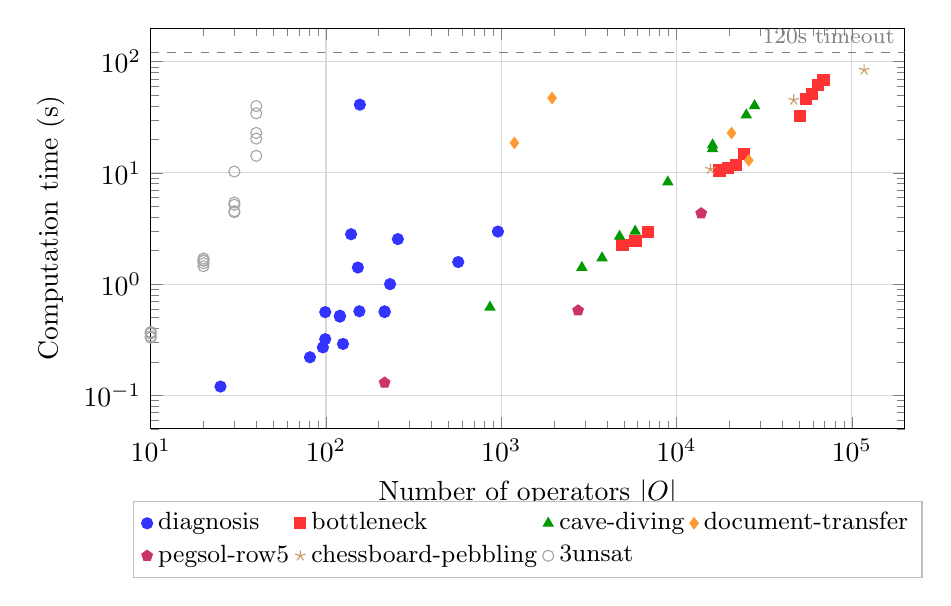
\begin{tikzpicture}
        \begin{axis}[
                xlabel={Number of operators $|O|$},
                ylabel={Computation time (s)},
                xmode=log,
                ymode=log,
                width=0.92\textwidth,
                height=0.55\textwidth,
                legend columns=4,
                legend style={
                        font=\small,
                        at={(0.5,-0.18)},
                        anchor=north,
                        draw=gray!50,
                        cells={anchor=west},
                    },
                grid=major,
                grid style={gray!30},
                xmin=10, xmax=200000,
                ymin=0.05, ymax=200,
                mark size=2pt,
            ]
            % diagnosis
            \addplot[only marks, mark=*, color=blue!80] coordinates {
                    (216,0.57) (216,0.56) (125,0.29) (568,1.58) (957,2.97)
                    (25,0.12) (81,0.22) (96,0.27) (156,41.09) (99,0.32)
                    (139,2.81) (99,0.56) (232,1.0) (152,1.41) (155,0.57)
                    (257,2.54) (120,0.51) (120,0.52)
                };
            \addlegendentry{diagnosis}
            % bottleneck
            \addplot[only marks, mark=square*, color=red!80] coordinates {
                    (4913,2.24) (5832,2.44) (6859,2.93) (17576,10.51)
                    (19683,10.98) (21952,11.81) (24389,14.86) (50653,32.65)
                    (54872,45.88) (59319,50.94) (64000,61.8) (68921,68.9)
                };
            \addlegendentry{bottleneck}
            % cave-diving
            \addplot[only marks, mark=triangle*, color=green!60!black] coordinates {
                    (4732,2.69) (3758,1.72) (2884,1.41) (862,0.62)
                    (27884,40.2) (16056,16.49) (24996,33.2) (16056,17.84) (8916,8.28)
                    (5806,2.99)
                };
            \addlegendentry{cave-diving}
            % document-transfer
            \addplot[only marks, mark=diamond*, color=orange!80] coordinates {
                    (25839,12.99) (20592,22.84) (1188,18.6) (1950,47.1)
                };
            \addlegendentry{document-transfer}
            % pegsol-row5
            \addplot[only marks, mark=pentagon*, color=purple!80] coordinates {
                    (216,0.13) (2744,0.58) (13824,4.33)
                };
            \addlegendentry{pegsol-row5}
            % chessboard-pebbling
            \addplot[only marks, mark=star, color=brown!80] coordinates {
                    (15625,10.82) (46656,45.22) (117649,84.34)
                };
            \addlegendentry{chessboard-pebbling}
            % 3unsat
            \addplot[only marks, mark=o, color=gray!70] coordinates {
                    (10,0.36) (10,0.34) (10,0.37) (10,0.33) (10,0.37)
                    (20,1.45) (20,1.62) (20,1.64) (20,1.7) (20,1.54)
                    (30,4.53) (30,4.44) (30,5.17) (30,10.29) (30,5.41)
                    (40,34.32) (40,39.92) (40,20.35) (40,22.87) (40,14.24)
                };
            \addlegendentry{3unsat}
            % timeout line
            \draw[dashed, gray] (axis cs:10,120) -- (axis cs:200000,120);
            \node[anchor=south east, font=\footnotesize, gray] at (axis cs:200000,120) {120s timeout};
        \end{axis}
    \end{tikzpicture}
    \caption{Computation time vs.\ operator count.}
    \label{fig:time_vs_ops}
\end{figure}
